\documentclass[a4paper,article,14pt]{extarticle}

% Подключаем главный пакет со всем необходимым
\usepackage{spbudiploma}

% Пакеты по желанию (самые распространенные)
% Хитрые мат. символы
\usepackage{euscript}
% Таблицы
\usepackage{longtable}
\usepackage{makecell}
% Картинки (можно вставлять даже pdf)
\usepackage[pdftex]{graphicx}

\usepackage{amsthm,amssymb, amsmath}
\usepackage{textcomp}

\usepackage{minted} % для примеров кода (требует параметра -shell-escape)
\usemintedstyle{bw}


\begin{document}

% Титульник в файле titlepage.tex
\newgeometry{left=30mm, top=20mm, right=15mm, bottom=20mm, nohead, nofoot}
\begin{titlepage}
\begin{center}

\textbf{Санкт--Петербургский государственный университет}\\
\textbf{Факультет математики и компьютерных наук}


\vspace{35mm}

\textbf{\textit{\large Остапенко Степан Сергеевич}} \\[8mm]
% Название
\textbf{\large Выпускная квалификационная работа}\\[3mm]
\textbf{\textit{\large Проверка выполнимости SMT-формул\\с помощью нейронных сетей}}

\vspace{20mm}
Уровень образования: бакалавриат\\
Направление 01.03.02 «Прикладная математика и информатика»\\
Основная образовательная программа СВ.5156.2020\\
«Современное программирование»\\[15mm]

% Научный руководитель, рецензент
\begin{flushright}
\begin{minipage}[t]{0.55\textwidth}
{Научный руководитель:} \\
доцент, \\
Факультет математики и \\
компьютерных наук СПбГУ, \\
к.ф.-м.н. Шалымов Дмитрий Сергеевич

\vspace{10mm}

{Рецензент:} \\
ведущий инженер ключевых проектов, \\
ООО «Техкомпания Хуавэй», \\
Ковальчук Сергей Валерьевич
\end{minipage}
\end{flushright}

\vspace{8mm}

{Санкт-Петербург}
\par{\the\year{} г.}
\end{center}
\end{titlepage}
\restoregeometry
\addtocounter{page}{1}


% Содержание
\tableofcontents
\pagebreak

\specialsection{Введение}

Введение широко представляет предметную область работы, указывает на место работы в научном или технологическом контексте.

\specialsection{Постановка задачи}

В постановке задачи коротко (по пунктам) указывается, что необходимо сделать в рамках работы.


\section{Обзорный раздел по предметной области}

\subsection{Использование формул}



Ненумерованная формула:

\begin{equation}
    \begin{pmatrix} \dot{\varphi}\\ \dot{\theta} \\ \dot{\psi} \end{pmatrix}
    = \begin{pmatrix}
        cos(\theta)cos(\psi) & -sin(\psi) & 0 \\
        cos(\theta)sin(\psi) & cos(\psi)  & 0 \\
        -sin(\theta)         & 0         &  1
    \end{pmatrix}^{-1}
    \begin{pmatrix} \omega_x\\ \omega_y \\ \omega_z \end{pmatrix}.
\end{equation}

Нумерованная формула:

\begin{equation}
    i^2 = -1.
    \label{eq:my_ref}
\end{equation}

Тест ссылки на формулу \ref{eq:my_ref}.

\subsection{Вставка рисунков}

\begin{figure}[ht]
\begin{center}
\scalebox{0.4}{
   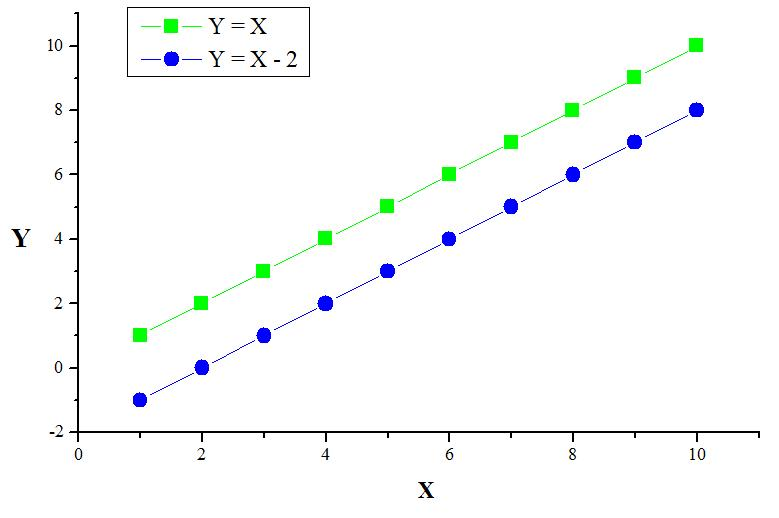
\includegraphics{images/graph.jpg}
}

\caption{
\label{graph-fig}
     Линейные функции.}
\end {center}
\end {figure}
Ссылаемся на график~\ref{graph-fig}.

\subsection{Ссылки на источники}

Ссылки на источники: \cite{voc}, \cite{vo2}, \cite{ij-sdk}.

\subsection{Оформление фрагментов кода}

В работах иногда приводят фрагменты кода:

\begin{minted}{kotlin}
fun main() {
    val name = "stranger"
    println("Hi, $name!")
    print("Current count:")
    for (i in 0..10) {
        print(" $i")
    }
}
\end{minted}


\subsection{Оформление таблиц}


\begin{table}[ht]
\begin{center}
\begin{tabular}{lccc}
    Имя & Работа 1 & Работа 2 & Итог \\
\hline
    Алиса & 8.0 & 9.0 & 8.5 \\
    Боб & 9.0 & 9.8 & 9.4 \\
    Чак & 9.1 & 9.3 & 9.2 \\
\end{tabular}
\caption{
\label{table-smth}
     Сравнение результатов.}
\end {center}
\end {table}

Ссылаемся на таблицу~\ref{table-smth}.




\section{Основной раздел}

\subsection{Подраздел}
\subsection{Подраздел}
\subsection{Подраздел}

\section{Основной раздел}

\subsection{Подраздел}
\subsection{Подраздел}
\subsection{Подраздел}

% !TEX root = ../main.tex


\section{Заключительный раздел с основными результатами}

\subsection{Подраздел}



\subsection{Подраздел}



\specialsection{Заключение}

Заключение должно подводить итоги работы и содержать информацию о полученных в рамках работы результатах.




% Аргумент {1} ниже включает переопределенный стиль с выравниванием слева
\begin{thebibliography}{1}
\bibitem{voc} D.W. Griffin, J.S.Lim. Multiband excitation vocoder. IEEE ASSP-36 (8), 1988, pp. 1223-1235.
\bibitem{vo2} A. Golovnev, A. S. Kulikov, I. Mihajlin. Families with Infants: Speeding Up Algorithms for NP-Hard Problems Using FFT., ACM Transactions on Algorithms, 12:3, 2016.
\bibitem{ij-sdk} IntelliJ Platform SDK. URL: \url{https://plugins.jetbrains.com/docs/intellij/welcome.html} (дата обр. 10.02.2022).
\end{thebibliography}
\end{document}